%----------------------------------------------------------------------------
\chapter{Results}
\label{chap:results}
%----------------------------------------------------------------------------

\section{Accuracy}
The best way to see the accuracy of the detector is through the webvisualizer.
The reader is encouraged to visit \url{https://najibghadri.com/msc-thesis/}
where you can interact with with the simulation playback and see each detection.

The reader might notice that most of the time the detected objects are located
closer than the ground truth. Recall, that the depth estimation happens on the
surface of the object. Estimating the centerpoint is difficult. If instead of
working with centerpoints I would have worked with a more complex approach of
first detection orientation or 3D bounding box, ther would be no need for
working with center points. I discuss improvements later on.

\begin{figure}[!ht]
	\centering
	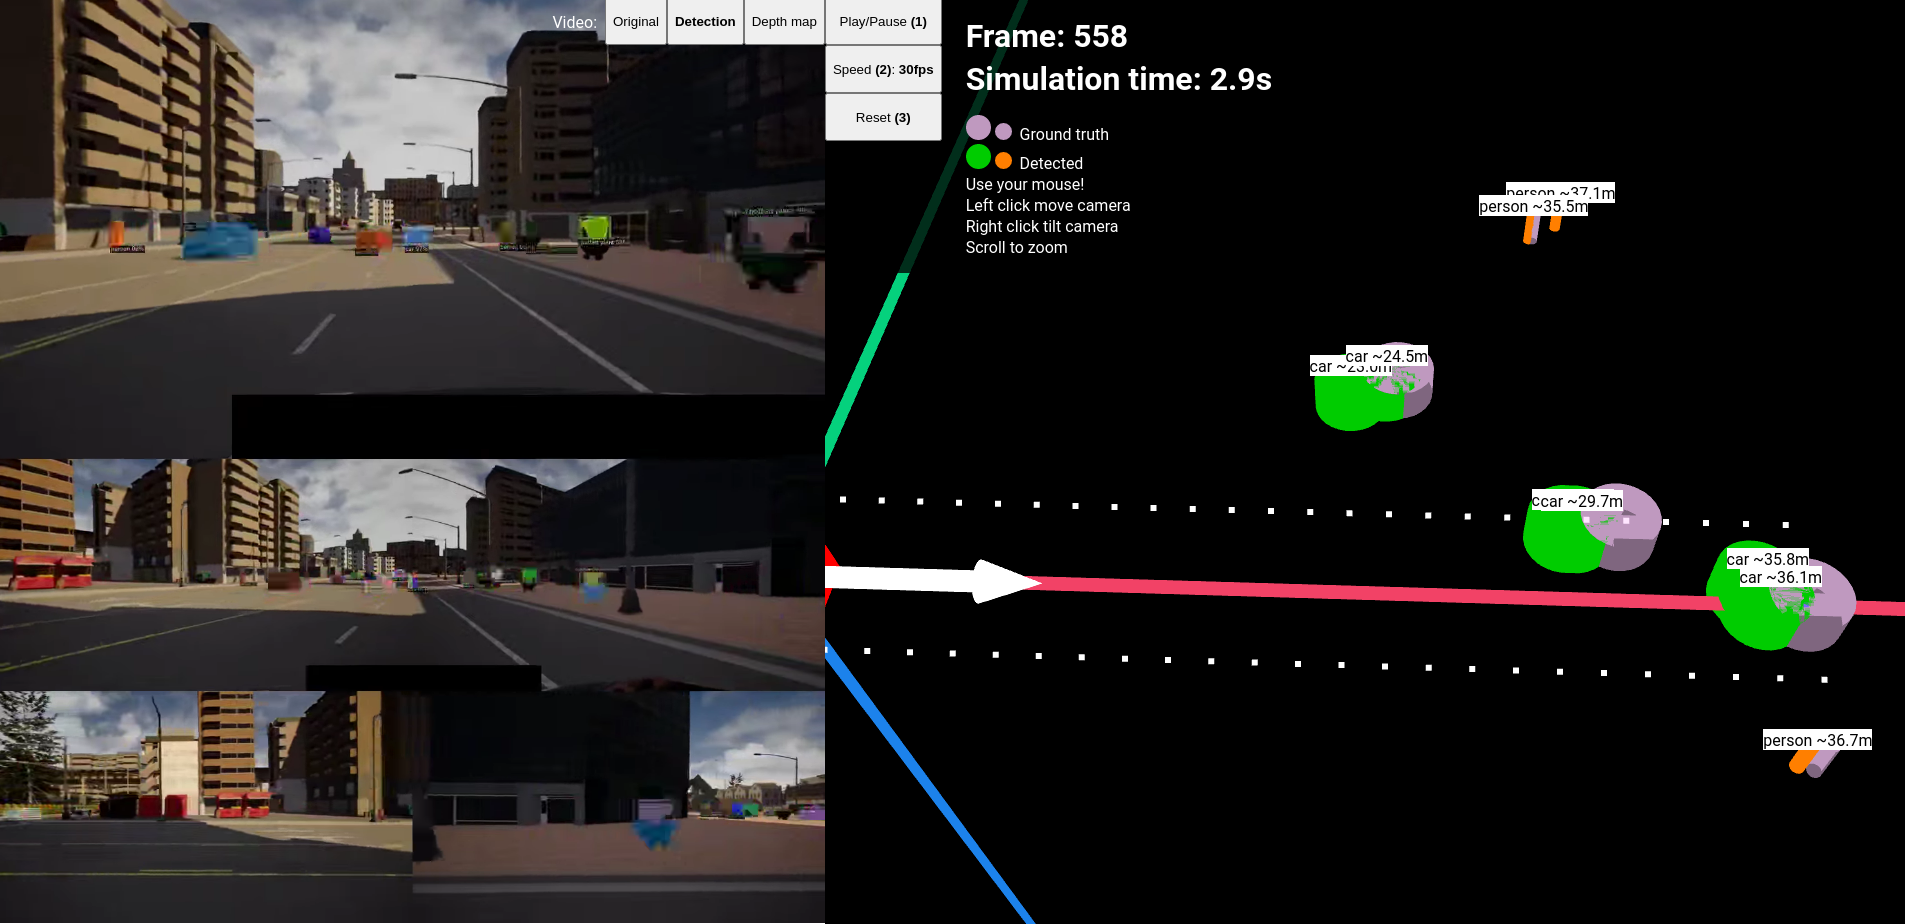
\includegraphics[width=150mm, keepaspectratio]{figures/accuracy.png}
	\caption{General accuraccy of the detector visualized in the webviewer}
	\label{fig:accuracy}
\end{figure}

Genearlly there are no missed objects but there are false positives. Most of the
detections are accurate within ~0.5meters. 

\begin{figure}[!ht]
	\centering
	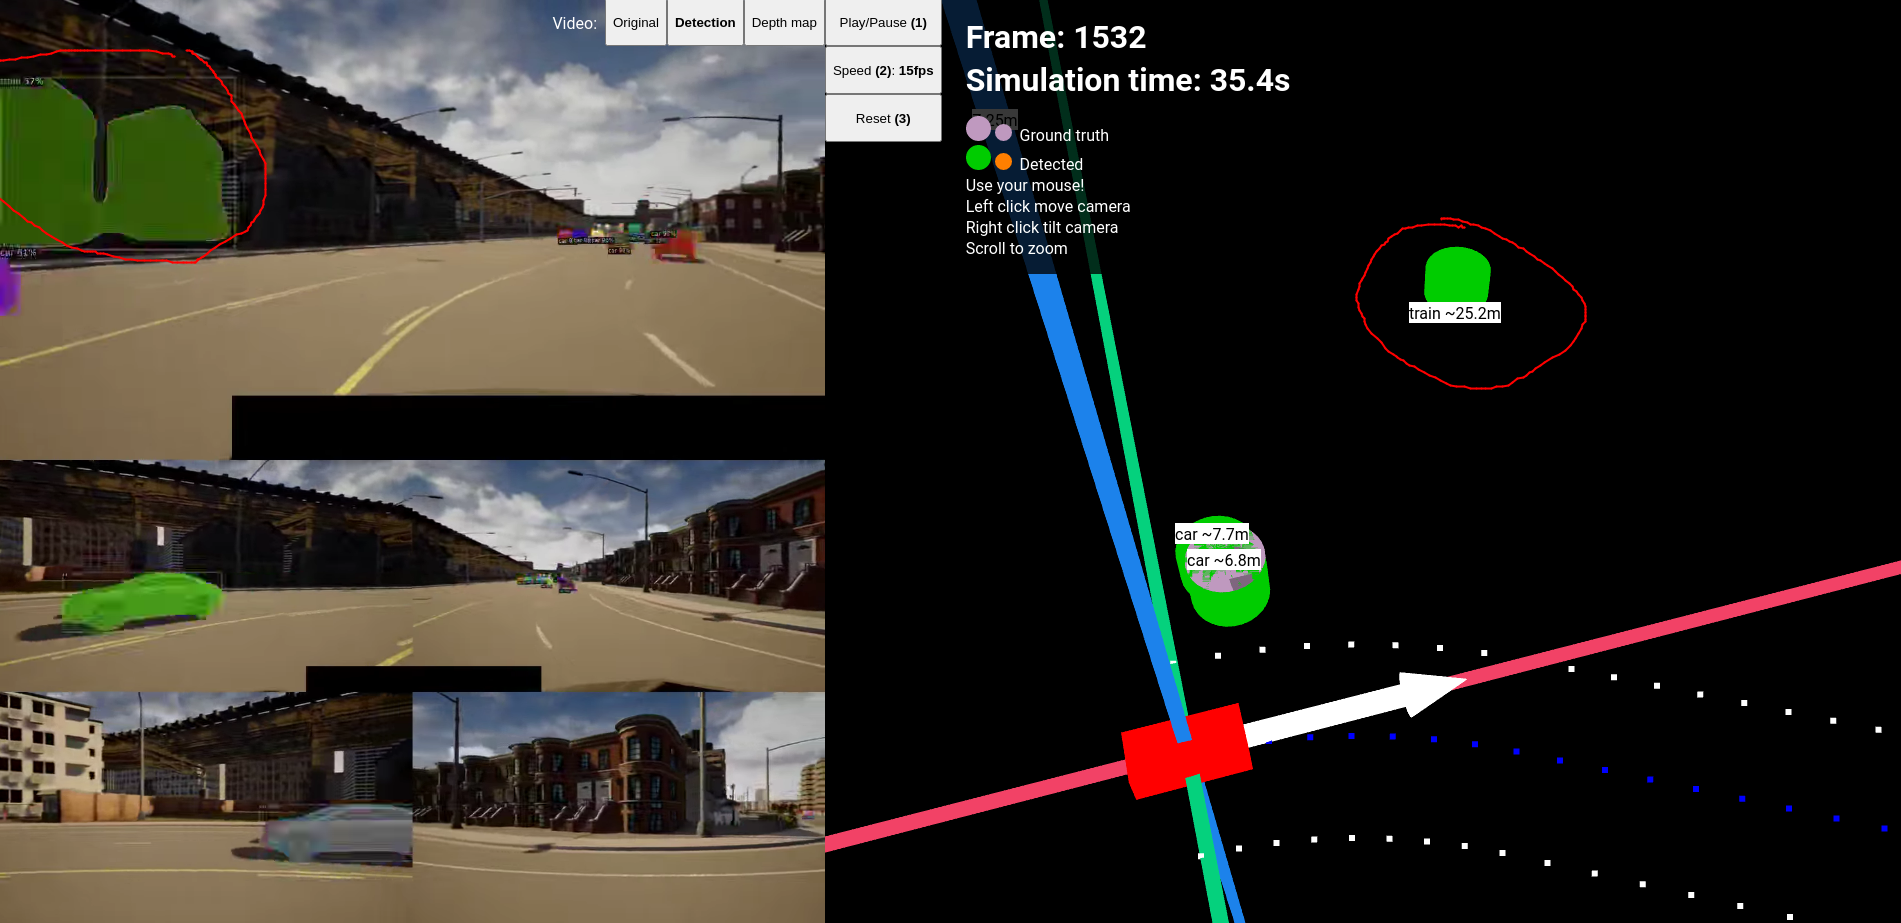
\includegraphics[width=150mm, keepaspectratio]{figures/accfalsepositive.png}
	\caption{False positive detection where a building is detected as a train}
	\label{fig:accfalsepositive}
\end{figure}


Depth estimation is not accurate enough due to the inaccuracy of the
blockmatching algorithm. This can be fixed with the use of LiDAR or radio
sensors instead of stereo imaging. Optimal sensor suite is discussed in
Improvements \autoref{chap:improvement}.

Since the setero sides overlap and they see different sides of the detect
objects in the detection log the objects appear as many times as many sides it
appears on as seen on \autoref{fig:accmultidet}. This can be fixed by using tracking and using a shared feature
dictionary. Another solution is to abandon stereo camera based depth estimation
and use mono cameras with radio or LiDAR sensors for depth estimation with
cameras having a small overlapping region. This would be similar to Tesla's
approach.

\begin{figure}[!ht]
	\centering
	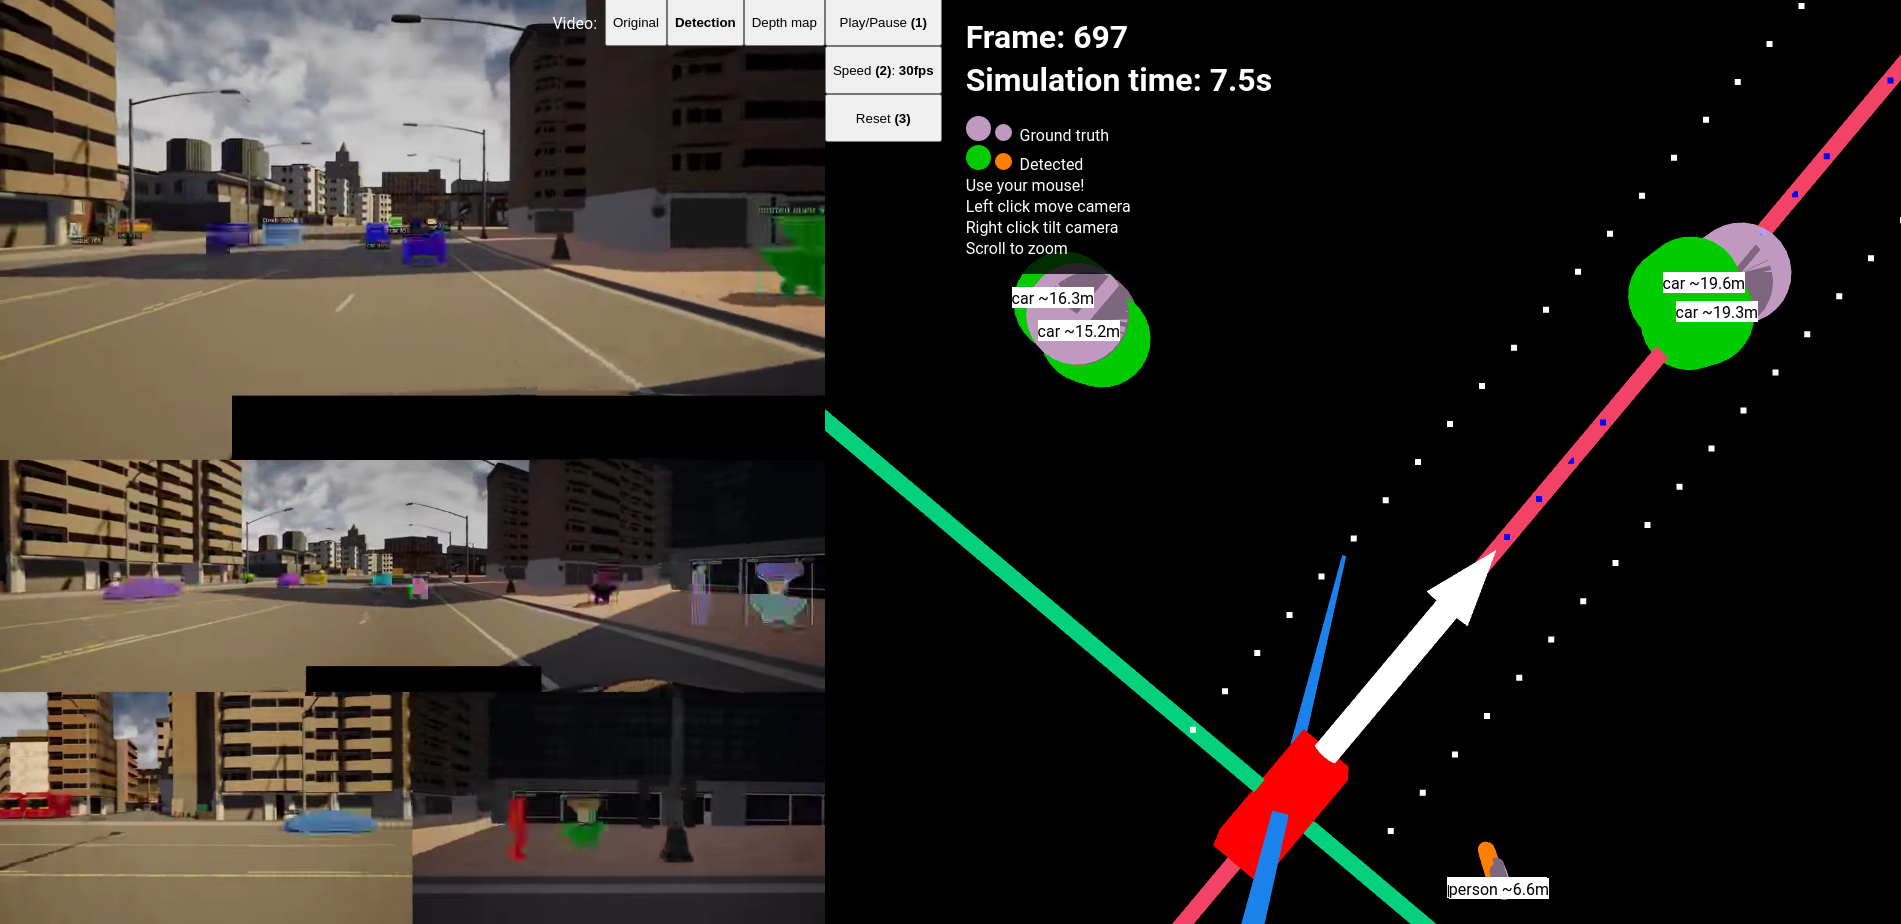
\includegraphics[width=150mm, keepaspectratio]{figures/accmultidet.png}
	\caption{Multiple detections of the same object due to overlapping stereo sides}
	\label{fig:accmultidet}
\end{figure}

Despite these depth estimation can be accurate to 70 meters even as seen on \autoref{fig:accfar}.
\begin{figure}[!ht]
	\centering
	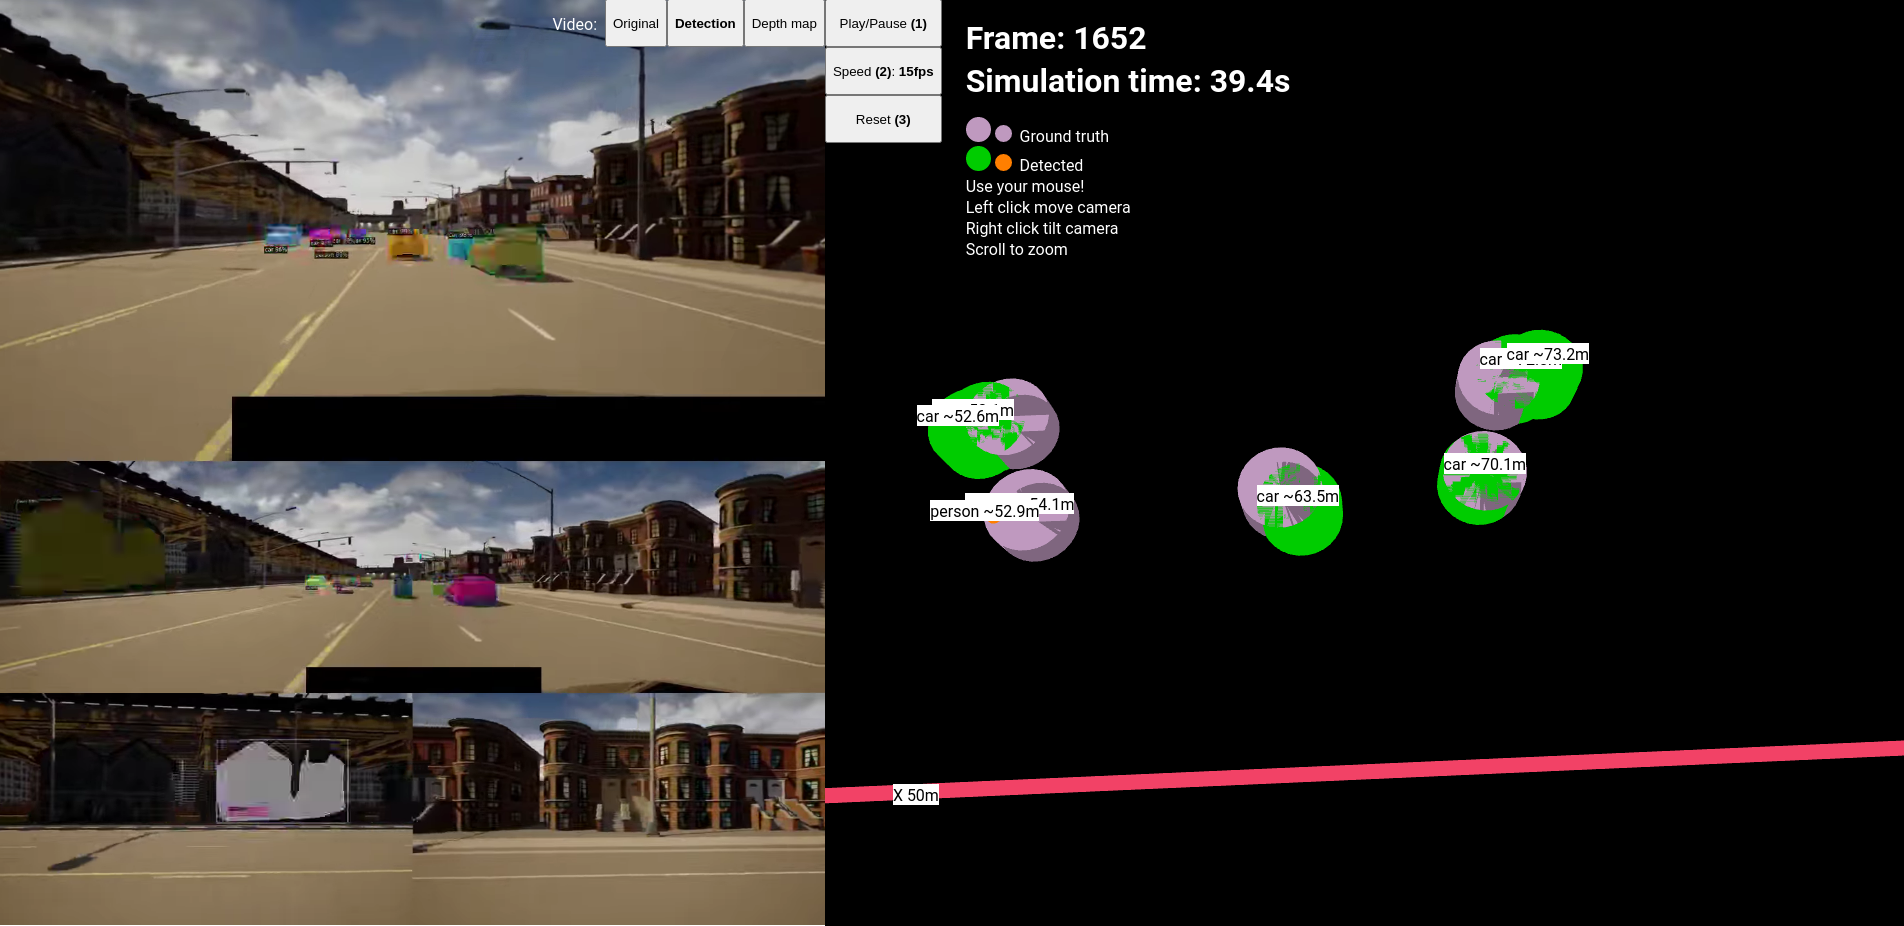
\includegraphics[width=150mm, keepaspectratio]{figures/accfar.png}
	\caption{Relatively accurate depth estimation for far distances of \textasciitilde70 meters}
	\label{fig:accfar}
\end{figure}

An automatic quantification method for the error will be discussed in \autoref{chap:improvement}.

\subsection{Fine tuning}
Choosing different convnet models for Detectron2 can change the performance and
accuracy of the detector. I used the ResNet-101
model~\cite{DBLP:journals/corr/HeZRS15}. ResNet50 is faster but I experienced
more detection misses.

\begin{table}[ht]
	\footnotesize
	\centering
	\begin{tabular}{ l c c }
		\toprule
		Sides       & FPS average \\
		\midrule
		All 5 sides & 0.53 FPS    \\
		One side    & 2.73 FPS    \\
		\bottomrule
	\end{tabular}
	\label{tab:TabularExample}
\end{table}

In \autoref{chap:improvement} imporvements on instance segmentation research
will be discussed that might lead to an improved detection speed over
Detectron2.

\section{Z coordinate ignored}
As discussed earlier in \autoref{chap:assumptions} about assumptions, the Z
coordinate (in Carla UE coordinates \autoref{fig:carlacoords}) is disgregarded
in the webvisualization. The accuracy of the Z coordinate is not worse or better
the X and Y coordinates but it doesn't add information and due to an
inconsistency in CARLA simulator when returning the location of actors for
vehicles and pedestriands the center point is interpreted differently. Hence it
showed a false inaccuracy in the Z direction, however not significant as seen on \autoref{fig:acczcoord}.

\begin{figure}[!ht]
	\centering
	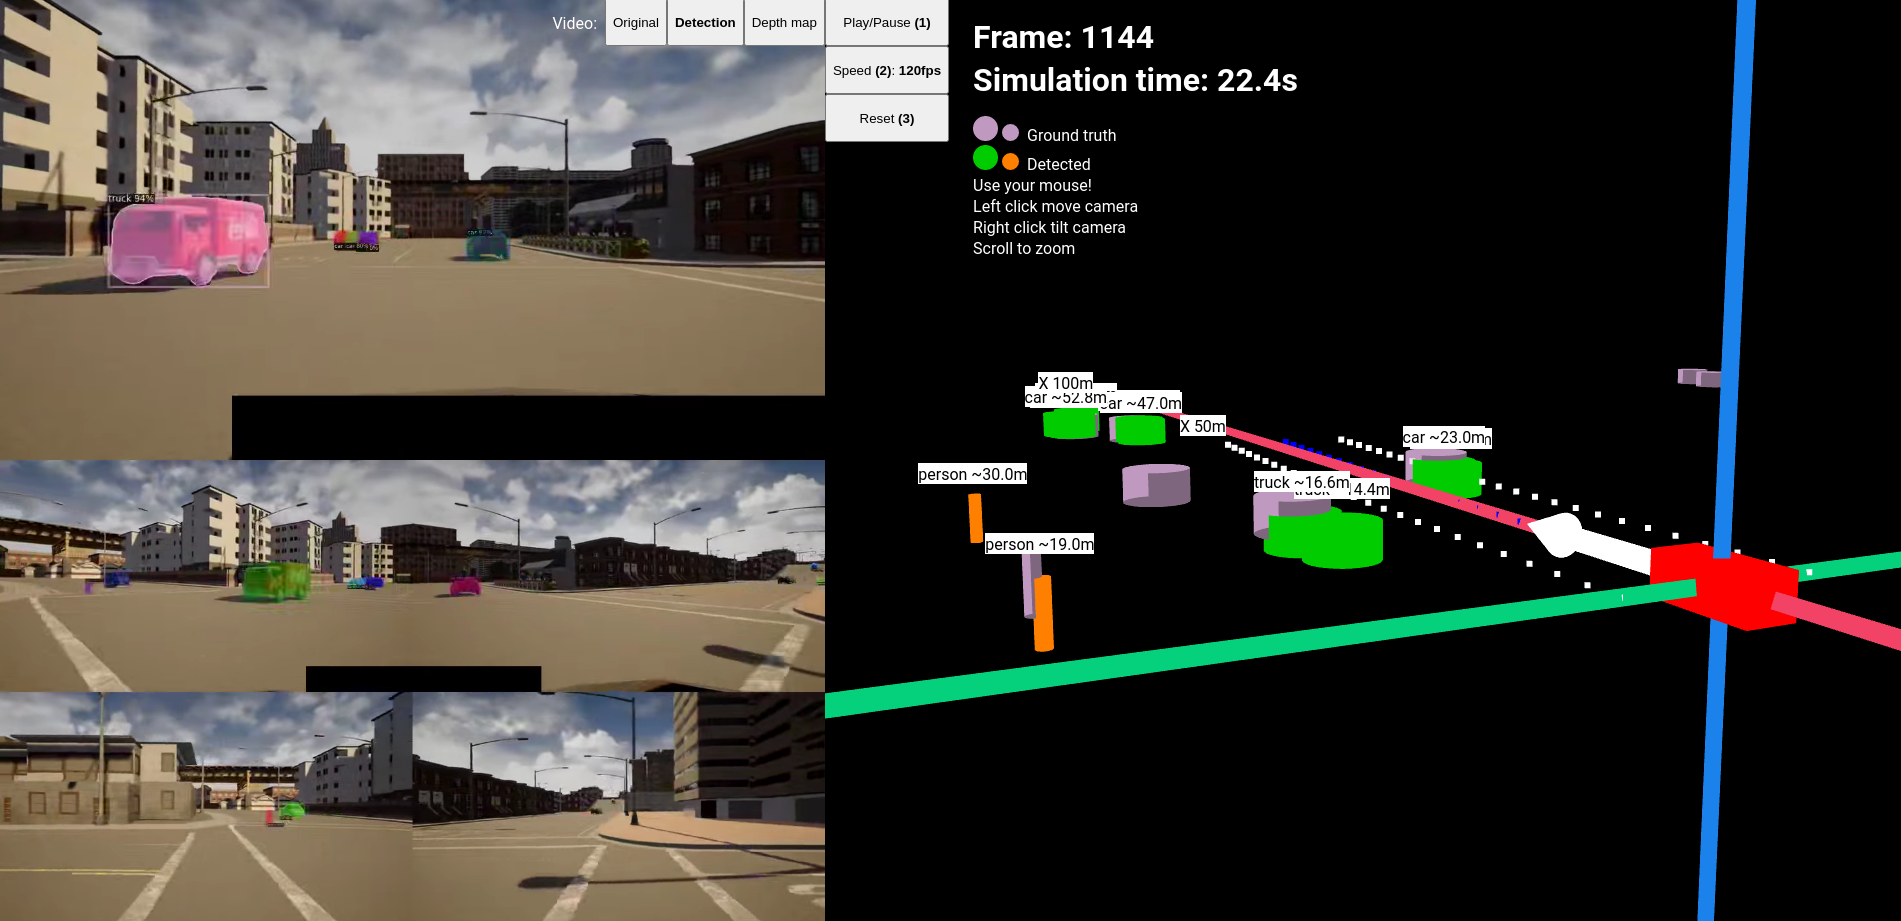
\includegraphics[width=150mm, keepaspectratio]{figures/acczcoord2.png}
	\caption{Inaccuracies on the Z coordinates are not significant}
	\label{fig:acczcoord}
\end{figure}

In \autoref{chap:improvement} on imporvements a different more complex and
robust approach to position estimation is discussed that doesn't use detected
bounding box centerpoints.

\section{Dark results}
There is only one map with a "night" situation, and it takes place in a city
that is well-luminated, hence I don't consider it a night light test, but it is
darker than other scenarios. The results are good no significant objects were
missed.

\begin{figure}[!ht]
	\centering
	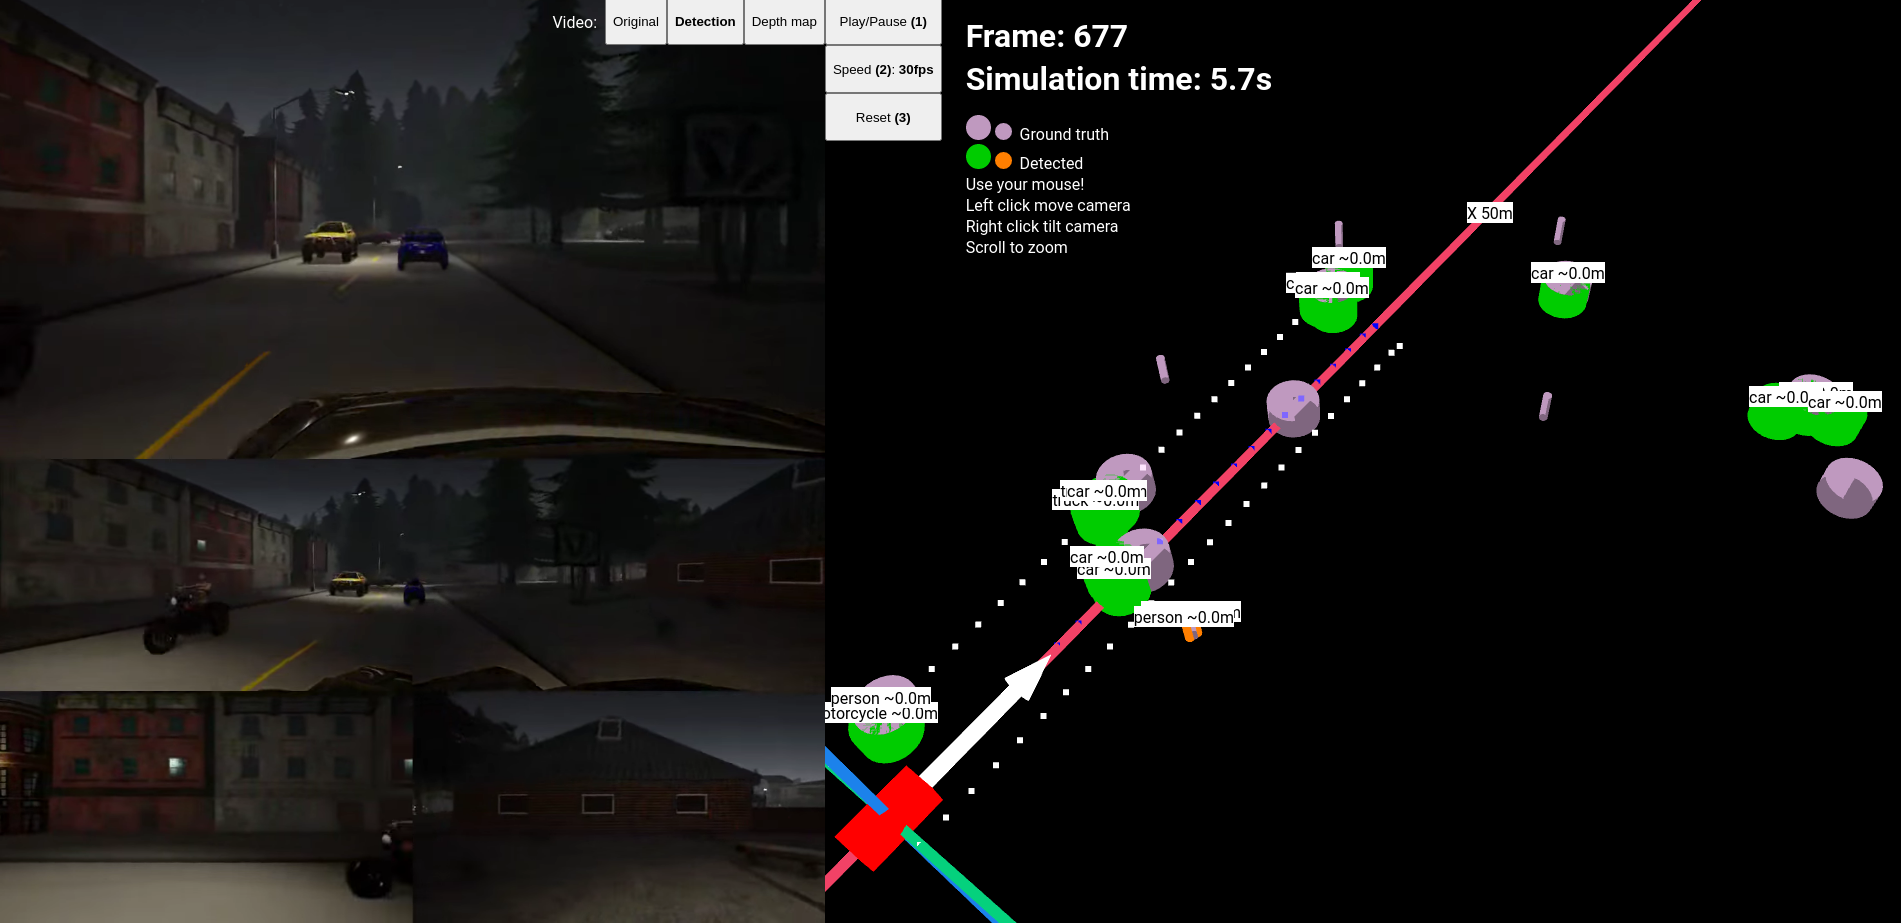
\includegraphics[width=150mm, keepaspectratio]{figures/nightresult.png}
	\caption{Night situation yields good performance}
	\label{fig:nightresult}
\end{figure}

\section{Hardware requirements}
It wasn't possible for me to evalute the real-timeness of the system simply
because the architecture doesn't allow that. As discussed earlier in
\autoref{chap:carlasim} Nvidia Drive Consteallation has support for HIL
simulation that could be used to test the real-timeness of systems.